\documentclass[12pt,a5paper]{article}

\usepackage[T1]{fontenc} % font encoding, lubab õ tähte kasutada
\usepackage[utf8]{inputenc} % oleme siiski 21. sajandis, vajadusel on ka olemas utf8x
\usepackage{lmodern} % lmodern ja micrtype käivad käsikäes, teeb teksti ilusamaks
\usepackage{microtype}
%\usepackage[estonian]{babel} % eesti keele poolitamisreeglid jpm
\usepackage[per=fraction, expproduct=cdot, decimalsymbol=comma]{siunitx} % http://www.bakoma-tex.com/doc/latex/siunitx/siunitx.pdf
\usepackage{graphicx}
\usepackage{wrapfig}
\usepackage{amssymb}
\usepackage{amsmath}
\usepackage{epstopdf} %minul on vaja, et .eps pilte saada
\usepackage{icomma} %koma arvust mõistlikul kaugusel
\usepackage{tikz}
\usepackage{tikzsymbols}
\usetikzlibrary{angles, quotes}
\usetikzlibrary{decorations.pathmorphing,patterns,arrows.meta}
\usepackage{float}

%paneme kõik mõõdud paika
\topmargin=-2.7cm \textheight=18.2cm \textwidth=12.77cm
\oddsidemargin=-1.5cm  \evensidemargin=-1.5cm
\setlength{\parindent}{0pt} \setlength{\parskip}{6pt} \sloppy

\relpenalty=10000 \binoppenalty=10000 % Tekstisisestes valemites reavahetusi ärgu olgu

\newcommand{\numb}[1]{\textbf{\large #1}}
\newcommand{\nimi}[1]{(\textsl{\small #1})}
\newcommand{\punktid}[1]{(\emph{#1~p.})}
\newcounter{ylesanne}
\newcommand{\yl}[1]{\addtocounter{ylesanne}{1}\newpage\numb{\theylesanne.} \nimi{\textbf{#1}} \newblock{}}
\newcommand{\pp}[1]{[\textbf{#1~p.}]}
\newcommand{\pv}[1]{\quad \hbox{[\textbf{#1~p.}]}}
\newcommand{\ue}[1]{\underline{\emph{#1}}}
\newcommand{\hence}{\quad \Rightarrow \quad}
\newcommand{\autor}[1]{\emph{ Autor: #1.\\}}
\newcommand{\lautor}[1]{\emph{ Lahenduse autor: #1.\\}}


\begin{document}

\begin{center}
  \textbf{\Large Eesti koolinoorte 68. füüsikaolümpiaad} \vspace{3pt}
  \emph{6. veebruar 2021. a. Piirkondlik voor.\\ \textbf{Gümnaasiumi} ülesannete lahendused}
\end{center}
\vspace{-10pt}
\numb{Eessõna}

Allpool on toodud iga ülesande üks õige lahenduskäik (mõnel juhul ka
enam). \textbf{Kõik alternatiivsed õiged lahenduskäigud tuleb hinnata samuti
maksimumpunktidega.} Iga alternatiivse lahenduskäigu jaoks tuleb
kontrollijatel koostada hindamisskeem, juhindudes võimalusel juuresoleva
hindamisskeemi punktijagamisproportsioonist. Soovituslikud
maha-arvamise punktid: numbriline arvutusviga --- 0,5; viga
teisendustes --- 0,5 p. (märgi jms väiksem viga) või 1 p. (viga, mis
viib dimensioonide konfliktini), maha arvata ainult üks kord, st
edasikanduvat viga mitte karistada; kui vastus tuleb füüsikaliselt
absurdne, siis võib täiendavalt karistada 0,5 punktiga; üksik viga
lähtevalemis: 0,5 p. (kui märgiviga) kuni 50\% (sisuline viga).
\vspace{20pt}

\yl{KUUL SFÄÄRIS}\punktid{8}\autor{Markus Rene Pae}
Läheme pöörlevasse taustsüsteemi. Siis mõjub kuulile kolm jõudu, raskusjõud, tsentrifugaaljõud ja toereaktsioon. Nende jõudude summa peab olema 0, sest pöörlevas taustsüsteemis seisab kuulike paigal. Sfääri pinna ja kuuli vahel puudub hõõrdejõud, seega on kuuli raskusjõu ning tsentrifugaaljõu summavektor sfääri raadiuse sihiline~\pp{1}.\par
Olgu $r$ kuulikese kaugus pöörlemisteljest. Sarnaste kolmnurkade tõttu, suhtuvad raskusjõu ja tsentrifugaaljõu teineteisesse kui $R-h$ ja $r$~\pp{1}. Seega peab kehtima seos:
$$ \frac{mg}{R-h} = \frac{m \omega^2 r}{r} \quad \pp2$$
kus $\omega$ on kuulikese ringsagedus. Viimase avaldise lihtsustamine ning sellest nurkkiiruse $\omega$ avaldamine annab:
$$ \omega = \sqrt{\frac{g}{R-h}} \quad \pp2$$
Kuna $\omega = \frac{2\pi}{T}$ \pp{1}, siis järelikult peab tiirlemise periood olema $T = 2 \pi \sqrt{\frac{R-h}{g}} \approx \SI{1.28}{\second}$ \pp{1}.

\begin{figure}[H]
	\centering
	\begin{tikzpicture}[scale=0.5]
    \coordinate (A) at (-5,0);
    \coordinate (O) at (0,0);
    \coordinate (kuul) at (-3,-4);
    \coordinate (base) at (0,-5);
    \coordinate (X) at (0,-4);

    % kauss
    \draw (A) arc (0:180:-5);

    % jooned
    \draw [dashed] (O) -- (0,-4) node[midway,right] {$R-h$};
    \draw (O) -- (-3,-4) node[midway,above,left] {$R$};
    \draw [dashed] (0,-4) -- (base) node[midway,right] {$h$};
    \draw [dashed] (O) -- (kuul);
    \draw [dashed] (X) -- (kuul) node[midway,below] {$r$};

    % jõud
    \draw[line width=2pt,blue,-stealth](kuul)--(-3,-8) node[anchor=north]{$mg$};
    \draw[line width=2pt,blue,-stealth](kuul)--(-6,-4) node[anchor=east]{$m\omega^2r$};
    \draw[line width=2pt,blue,-stealth](kuul)--(O) node[anchor=south west]{};

    % kuul
    \node[circle,fill=black,inner sep=1mm] at (kuul) {};
  \end{tikzpicture}
\end{figure}


\yl{KLAASPUDEL}\punktid{8}\autor{Kaur Aare Saar}
Kõige suurem rõhk on pudelis siis, kui kogu jää on ära jäätunud ning pudeli temperatuur on $T_1=\SI{0}{\celsius}$ \pp{1}. \par
Et maksimeerida pudelis olevat vee kogust, peab rõhk just siis olema maksimaalne võimalik. Maksimaalne rõhk pudelis on välise rõhu ja maksimaalse ülerõhu summa $p=p_0+3p_0=4p_0$~\pp1. \par
Algul on õhku pudelis $V-V_{\text{v}}$. Ideaalgaasi seadusest saame, et pärast peab pudelis oleva õhu ruumala olema
$$(V-V_{\text{v}})\frac{p_0T}{pT_0}=(V-V_{\text{v}}) \frac{T}{4T_0} \quad \pp2.$$
Kui kogu vesi on ära jäätunud, siis jää ruumala on $V_{\text{j}}=V_{\text{v}}\frac{\rho_{\text{v}}}{\rho_{\text{j}}}$~\pp1. \par
Kuna pudeli ruumala ei muutu, siis saame
$$V=V_{\text{v}}\frac{\rho_{\text{v}}}{\rho_{\text{j}}} + (V-V_{\text{v}}) \frac{T}{4T_0} \quad \pp2$$
Siit saame avaldada $V_{\text{v}}$:
$$V_{\text{v}}=V \frac{1-\frac{T}{4T_0}}{\frac{\rho_{\text{v}}}{\rho_{\text{j}}}-\frac{T}{4T_0}} = \SI{0.90}{\liter} \quad \pp1$$

\yl{JOOGID}\punktid{8}\autor{Kaarel Hänni}
Osas (a) antud jooke ei ole võimalik kokku segada. Esiteks on ilmselge, et mitme järjestikuse segamise tulemusel saadud jooki saab valmistada ka kolmest anumast sellesse jooki pandud veekoguste ühekordse segamisega~\pp{0,5}.\par
Näitame nüüd, et nii pole aga võimalik valmistada $\SI{1.5}{\kilo\gram}$ jooki temperatuuril $\SI{13}{\celsius}$. Oletame, et sellise joogi saab valmistada segades koguse $x$ vedelikku temperatuuril $\SI{10}{\celsius}$ ja koguse $y=\num{1.5}-x$ vedelikke temperatuuril vähemalt $\SI{20}{\celsius}$~\pp{1,5}. Sellisel juhul
\begin{align*}
x\cdot 10+y\cdot 20 &\leq 1.5\cdot 13 \\
10x+30-20x &\leq 19.5 \\
10.5 &\leq 10 x \\
x &> 1,
\end{align*}
aga algselt oli temperatuuril $\SI{10}{\celsius}$ vett ainult $\SI{1}{\kilo\gram}$, seega $x\leq 1$ ja viimane võrratus on võimatu \pp2.

Osas (b) antud jooke ei ole võimalik kokku segada, sest energiat oleks lõpus vähem kui alguses. Seda saab näha järgnevalt. Energia jäävuse tõttu peab enne ja pärast segamist vee keskmine temperatuur olema sama \pp{1}. Algselt on keskmine temperatuur $$\frac{\SI{10}{\celsius} \cdot \SI{1}{\kg} +\SI{20}{\celsius} \cdot \SI{1}{\kg}+\SI{30}{\celsius} \cdot \SI{1}{\kg}}{3\text{kg}}=\SI{20}{\celsius}.  \quad \pp{1}$$
Pärast selliste jookide segamist oleks ülejäänud $3-5\cdot 0.5=\SI{0.5}{\kilo\gram}$ vett temperatuuril ülimalt $\SI{30}{\celsius}$, sest see oli kõrgeim algne temperatuur)~\pp{1}. \par
Seetõttu on vee keskmine temperatuur pärast selliste jookide segamist ülimalt
$$\frac{\SI{0.5}{\kg}\cdot(\SI{12}{\celsius} +\SI{17}{\celsius} +\SI{18}{\celsius}+\SI{20}{\celsius} +\SI{22}{\celsius}+\SI{30}{\celsius})}{\SI{3}{\kg}}=\SI{19.8}{\celsius},$$
mis on vähem kui algne keskmine temperatuur \pp1. Seega selliseid jooke ei saa segada.

\yl{BATÜSKAAF}\punktid{8}\autor{Kaido Reivelt}
Kuna kasutada on lihtmehhanismid, pole maksimaalne rakendatav jõud oluline, sest Monikal on neid kasutades võimalik avaldada ükskõik kui suuri jõude. Rõhu vahe batüskaafi väljas ja sees on
$$\Delta p=\rho gh. \quad \pp{2}$$

Rõhuvahe avaldab silindrile jõudu
$$F_p=\Delta p S = \rho gh S. \quad \pp{2}$$
Sellise jõuga tuleb tööd teha, et vett batüskaafist välja pumbata. Vee välja pumpamiseks vajalik töö avaldub kui
$$A=F_p\cdot \Delta x= \rho gh S \Delta x. \quad \pp{2}$$

Paneme tähele, et batüskaafist on tarvis välja pumbata kokku $V=\SI{1}{\liter}$ vett, järelikult peab kehtima $V=S\Delta x$ \pp{1}.

Ruumala $V$ batüskaafist välja pumpamiseks on vaja teha tööd $A=\rho g h V$. Kuna teame, et tööd saab teha keskmise võimsusega $P=\SI{100}{\W}$, saame et vee välja pumpamiseks kulub
$$t=\frac{A}{P}=\frac{\rho g h V}{P}=\SI{1009}{\s}. \quad \pp{1}$$

\yl{VOOLUALLIKAS}\punktid{8}\autor{Jaan Toots}
Olgu pinge koormise klemmidel (ja ühtlasi ka sisetakisti klemmidel) $V$.
Siis voolutugevus läbi koormise on $I = I_0 - \frac VR$ \pp2. Seega võimsus on
$$P = IV = I_0V - \frac{V^2}R \quad \pp3$$
Järelikult võimsus koormisel avaldub kui ruutfunktsioon pingest. Selle ruutfunktsiooni maksimumi leidmiseks viime võimsuse avaldise kujule
$$P=-\frac1R \left(V - \frac{I_0R}2\right)^2 + \frac{I_0^2R}4 \quad \pp2$$
Paneme tähele, et $R>0$ ja $(V - \frac{I_0R}{2})^2 \ge 0$. \par
Seega on maksimaalne võimsus $P_0 = \frac{I_0^2R}{4}$ \pp1 ja seda pingel $V = \frac{I_0R}{2}$.



\yl{JALGRATTUR}\punktid{10}\autor{Jarl Patrick Paide}
Joonisel punane joon kirjeldab jalgratturi asukohta $s$ ajahetkel $t$ (Rattur läbib teelõigu pikkusega $L$ aja $T$ jooksul). Auto alustab sõitu juhuslikul ajahetkel $0 < t_a < T$ ja juhuslikust kohast $0 < s_a < L$. Kui auto alustab sõitu jalgratturist eespool siis ei sõida auto jalgratturist mööda \pp{2}. Jalgrattur sõidab poole auto kiirusega. Seetõttu ei jõua auto jalgratturist mööda kui auto alustab sõitu vähemalt kaks korda kaugemal lõpule kui jalgratturi kaugus lõpuni \pp{2}. Seega auto sõidab jalgratturist mööda, kui auto alustab sõitu jalgratturist tagapool ja kui auto on jalgratturile lähemal kui jalgrattur lõppule. Vastavalt sobiv vahemik on näidatud joonisel sinise alana. Kui auto algpunkt $(t_a; s_a)$ asub sinisel alal siis sõidab auto jalgratturist mööda.

\begin{figure}[H]
  \centering
  \begin{tikzpicture}[domain=0:4]
    \draw[->] (0,0) node[below] {0} -- (2,0) node[below] {$\frac{T}{2}$} -- (4,0) node[below] {$T$} -- (4.2,0) node[right] {$t$};
    \draw[->] (0,0) node[left] {0} -- (0,4) node[left] {$L$} -- (0,4.2) node[above] {$s$};
    \draw[dashed] (0,4) -- (4,4) -- (4,0);
    \fill[fill=blue!30] (0,0) -- (2,0) -- (4,4);
    \draw[dotted] (2,0) -- (2,4);
    \draw[color=red] plot (\x,\x);
  \end{tikzpicture}
\end{figure}


Tõenäosus, et auto sõidab jalgratturist mööda on võrdne sinise ala suhetega kogu pindalasse.
$$\frac{(L\times \frac T2)/2}{L \times T} = \frac{1}{4} \quad \pp{6}$$

Alternatiivselt saab vastuse leida ka ilma jooniseta. Sellisel juhul anda punkte arvutuste eest järgnevalt. Tõenäosus, et auto alustab sõitu jalgratturist eespool on $\frac{1}{2}$ \pp{2}. Tõenäosus, et auto alustab sõitu jalgratturist tagapool ja ei möödu jalgratturist on $\frac{1}{4}$ \pp{3}. Seega tõenäosus, et auto sõidab jalgratturist mööda on  $\frac{1}{4}$ \pp{1}.

\yl{RIPPUV LAENG}\punktid{10}\autor{Kaur Aare Saar}
Selleks, et rippuv laeng püsiks paigal, peab talle mõjuvate jõuvektorite summa olema $0$. Rippuvale laengule mõjub kolm jõudu, raskusjõud $mg$, nööri pinge $T$ ning laengute vaheline elektrostaatiline jõud $F$. \pp1

\begin{figure}[H]
	\centering
	\begin{tikzpicture}[scale=1.5]
    \coordinate (A) at (0,0);
    \coordinate (q1) at (1,-2);
    \coordinate (q2) at (0,-4);
    \coordinate (D) at (1,-0);
    \coordinate (E) at (0.5,-1);
    \coordinate (F) at (1.5,-1);
    \coordinate (G) at (1,-4);

    % kinnitus
    \fill [pattern = north east lines] (-0.5,0) rectangle (0.5,0.2);
    \draw[thick] (-0.5,0) -- (0.5,0);

    %nöör
    \draw [thick] (q1)	-- (A) node[yshift=-1.2cm,xshift=0.9cm] {$L$};

    %abijooned
    \draw [dashed] (q2) -- (A) node[midway,left] {$2h$};
    \draw [dashed] (q1) -- (q2) node[midway, right] {$L$};
    \draw [dashed] (q1) -- (D) node[right,yshift=-1.2cm] {$h$};

    %jõud
    \draw[line width=2pt,blue,-stealth](q1)--(E) node[anchor=north east]{$T$};
    \draw[line width=2pt,blue,-stealth](q1)--(F) node[anchor=north west]{$F$};
    \draw[line width=2pt,blue,-stealth](q1)--(G) node[anchor=north west]{$mg$};

    %nurgad
    \draw pic [text="$\theta$", draw, angle radius=1.1cm] {angle=q2--A--q1};
    \draw pic [text="$\theta$", draw, angle radius=1.05cm] {angle=D--q1--A};
    \draw pic [text="$\theta$", draw, angle radius=1.1cm] {angle=F--q1--D};    

    %laengud
    \node[circle,fill=black,inner sep=1mm] at (q1) {};
    \node[circle,fill=black,inner sep=1mm] at (q2) {};
  \end{tikzpicture}
\end{figure}

Paneme tähele, et kinnituskoht, rippuv laeng ning fikseeritud laeng moodustavad võrdhaarse kolmnurga, mistõttu on laengute vaheline kaugus~$L$~\pp1.

Seega laengute vaheline elektrostaatiline jõud on:
$$F=\frac{kq_1q_2}{L^2} \quad \pp1$$

Raskusjõul puudub horisontaalkomponent. Järelikult on elektrostaatilise jõu ja nööri pinge horisontaalkomponendid võrdsed ja vastassuunalised \pp1.

Seega kuna elektrostaatilise jõu ja nööri pinge horisontaalkomponendid on võrdsed, siis sümmeetria tõttu on need jõud absoluutväärtuselt võrdsed $T=F$ \pp1.

Nüüd vertikaalsuunalisest jõudude tasakaalust saame
$$mg=T\cos\theta + F\cos (-\theta) = 2F\cos\theta = 2 \cos\theta \frac{kq_1q_2}{L^2} \quad \pp3,$$
kus $\theta$ on nurk vertikaalsihi ja nööri vahel.
Täisnurksest kolmnurgast saame $\cos\theta = \frac hL$ \pp1.

Nüüd asendades sisse $\cos\theta$ vertikaalsuunalise jõudude tasakaalu võrrandisse ja avaldades sealt $m$, saame
$$m=\frac{2kq_1q_2h}{gL^3} \quad \pp1$$

\yl{LAINEJUHT}\punktid{10}\autor{Hans Daniel Kaimre}
\begin{center}
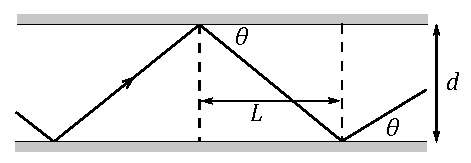
\includegraphics[]{lainejuht_lah.pdf}
\end{center}

Kaod sellises lainejuhis tulenevad tõsiasjast, et iga peegeldusega läheb kaduma pisut valgust, kuna peegeldub vaid $R=\SI{99.8}{\percent}$ sellest \pp{1}. Kui valgus levib lainejuhi telje sihis kahe peegelduse vahel $L$ võrra (vt joonist), saame intensiivsuse sõltuvuse levimise distantsist $l$ panna kirja kujul
$$I=I_0 R^{l/L} \quad \pp{2}$$
kust
$$ \ln \frac{I}{I_0}=
\frac{l}{L}  \cdot \ln R=
\ln R \cdot\frac{l}{d}\tan\theta
\quad \Rightarrow \quad
l = \frac{\ln\frac{I}{I_0}}{\ln R}\cdot\frac{d}{\tan\theta}
\quad \pp{2}$$

Meile pole teada ei $d$ ega $\theta$, küll saame need leida. Tuletatud seosest on näha, et valgus levib kaugemale, kui $\theta$ on võimalikult väike \pp{1}. Ülesande püstituses antud graafikult võib näha, et $\theta$ minimaalne võimalik väärtus on \SI{1.3}{\degree} (sellele vastab $N=1$) \pp{1}. Kasutades ülesande püstituses antud seost, saame
$$d = \frac{N\lambda}{2\sin\theta}=\frac{1\cdot\SI{1.55}{\micro\m}}{2\cdot\sin(\SI{1.3}{\degree})}=\SI{34}{\micro\m}. \quad \pp{1}$$
Kui valguse intensiivsus on vähenenud 10 korda, $\frac{I}{I_0}=0.1$ \pp{1} ning sellele vastavaks levimise distantsiks saame
$$l=\frac{\ln(\num{0.1})}{\ln(\num{0.998})}\cdot\frac{\SI{34}{\micro\m}}{\tan(\SI{1.3}{\degree})}=\SI{1.7}{\m}. \quad \pp{1}$$
Nagu näha, väheneb valguse intensiivsus väga kiirelt. Seetõttu kasutataksegi modernsetes süsteemides signaali edastamiseks fiibreid, kus täieliku sisepeegeldumise tõttu kadusid pole. Tänapäevaste optiliste fiibritega toimub signaali tugevuse 10-kordne vähenemine umbes 50 kilomeetriga.

\yl{KIIRUSE KUJUTIS}\punktid{12}\autor{Jaan Kalda}
Valgusallika kiirusvektor ja kujutise kiirusvektor defineerivad kaks sirget, millest üks on teise kujutis. Need lõikuvad teadupärast läätse tasandil. Pikendades kiirusvektoreid lõikumiseni leiame nimetatud sirgete lõikepunkti $E$, mis asub läätsel. \pp3 \par
Valgusallikat ja selle kujutist ühendav sirge $AB$ peab läbima läätse keskpunkti. \pp1 \par
Sama peab kehtima sirge jaoks, mis ühendab valgusallika ja kujutise asukohti hästi lühikese ajavahemiku pärast. Üks võimalus ongi märkida valgusallika ja kujutise asukohad lühikese ajavahemiku $\Delta t$ pärast --- sellistes punktides $A'$ ja $B'$, kus nihkevektorid  $\vec{AA'}$ ja $\vec{BB'}$ on võrdelised vastavate kiirusvektoritega. \pp3 \par
Sellisel juhul saame leida läätse keskpunkti kui sirgete $AB$ ja $A'B'$ lõikepunkti. \pp2 \par
Probleem on selles, et niimoodi leitud asukoht on ebatäpne, sest kaks sirget lõikuvad väga väikese nurga all. Oluliselt täpsema tulemuse saame, kui paneme tähele, et projitseerides nihkevektorid $\vec{AA'}$ ja $\vec{BB'}$ sirge $AB$ ristsihile vektoriteks $\vec{AA''}$ ja $\vec{BB''}$ saame sirge $A''B''$, mis  lõpmatult lühikeste nihete puhul ühtib sirgega $A'B'$ ja mille lõikepunkt $O$ sirgega $AB$ püsib liikumatuna ka suurte nihete korral. Seetõttu võime punkti $O$ leidmiseks projitseerida kiirusvektorite lõpp-punktid sirge $AB$ ristsirgetele punktideks $C$ ja $D$. Sellisel juhul on punkt $O$ sirgete $AB$ ja $CD$ lõikepunktiks. \pp2 \par
Läätse tasandiks on sirge $OE$ ja läätse keskpunktiks punkt $O$ \pp1.
\begin{figure}[H]
  \centering
  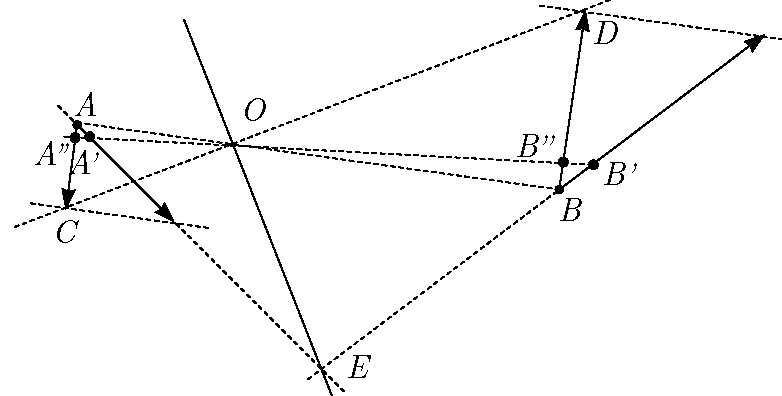
\includegraphics[width=0.69\textwidth]{lxxts-kiirused-lahendus.pdf}
\end{figure}

\emph{Märkus:} \\
Väide, et punkt $A'$ kujutub punktiks $B'$ kehtib ainult siis, kui punktid $A'$ ja $B'$ paiknevad lõpmata lähedal vastavalt punkidele $A$ ja $B$. Valgusallika kiirusvektori otspunkt ei kujutu kujutise kiirusvektori otspunktiks. Kui punktvalgusallikas liigub ise konstantse kiirusega, siis ei saa sama väita tema kujutise kiiruse kohta. Alloleval joonisel on kujutatud siniste täppidega konstantse kiirusega liikuva valgusallika asukohad võrdsete ajavahemike tagant ning punaste täppidega vastavate siniste täppide kujutised. Jooniselt on näha, et punased täpid ei paikne võrdsete vahedega, järelikult kujutis ei liigu konstantse kiirusega.

\begin{figure}[H]
  \centering
  \begin{tikzpicture}[scale=0.3]
    \draw[{<[scale=1.6]}-{>[scale=1.6]}] (0.60294118, 10.20588235) -- (9.27941176, -11.44117647);
    \draw (-2.2745098 , -3.50980392) edge[dashed] (26.58823529,  8.05882353);
    \filldraw [blue]
    (0.0, 0.0) circle (3pt)
    (0.25, -0.25) circle (3pt)
    (0.5, -0.5) circle (3pt)
    (0.75, -0.75) circle (3pt)
    (1.0, -1.0) circle (3pt)
    (1.25, -1.25) circle (3pt)
    (1.5, -1.5) circle (3pt)
    ;
    \filldraw [red]
    (16.0, -2.0) circle (3pt)
    (16.65056497175141, -1.5353107344632768) circle (3pt)
    (17.470625798212005, -0.9495530012771394) circle (3pt)
    (18.5363436123348, -0.1883259911894275) circle (3pt)
    (19.977547495682206, 0.8411053540587212) circle (3pt)
    (22.035115303983222, 2.310796645702305) circle (3pt)
    (25.212, 4.58) circle (3pt)
    ;
  \end{tikzpicture}
\end{figure}

\yl{LAEVA VETTELASKMINE}\punktid{12}\autor{Päivo Simson}
\textbf{Lahendus 1.} \\
Laevale mõjuvad raskusjõud $m\overrightarrow{g}$, kaldpinna toereaktsioon $\overrightarrow{N}$, hõõrdejõud $\overrightarrow{F}_h$ ja köie tõmbejõud $\overrightarrow{T}$. Et laev paigal püsiks, peab nende jõudude vektorsumma võrduma nulliga. Raskusjõud $m\overrightarrow{g}$ on konstantne suurus. Köie tõmbe kaldpinnaga ristuv komponent võib toereaktsiooni suurendada või vähendada ja vastavalt seosele $F_h=\mu N$ suureneb või väheneb samas proportsioonis ka hõõrdejõud. See tähendab, et vektori $\overrightarrow{N}+\overrightarrow{F}_h$ siht ei sõltu köie tõmbest $\overrightarrow{T}$, sest $\tan\gamma=F_h/N=\mu=\textit{const}$.

\begin{figure}[h]
\vspace{-0.0cm}
  \begin{center}
    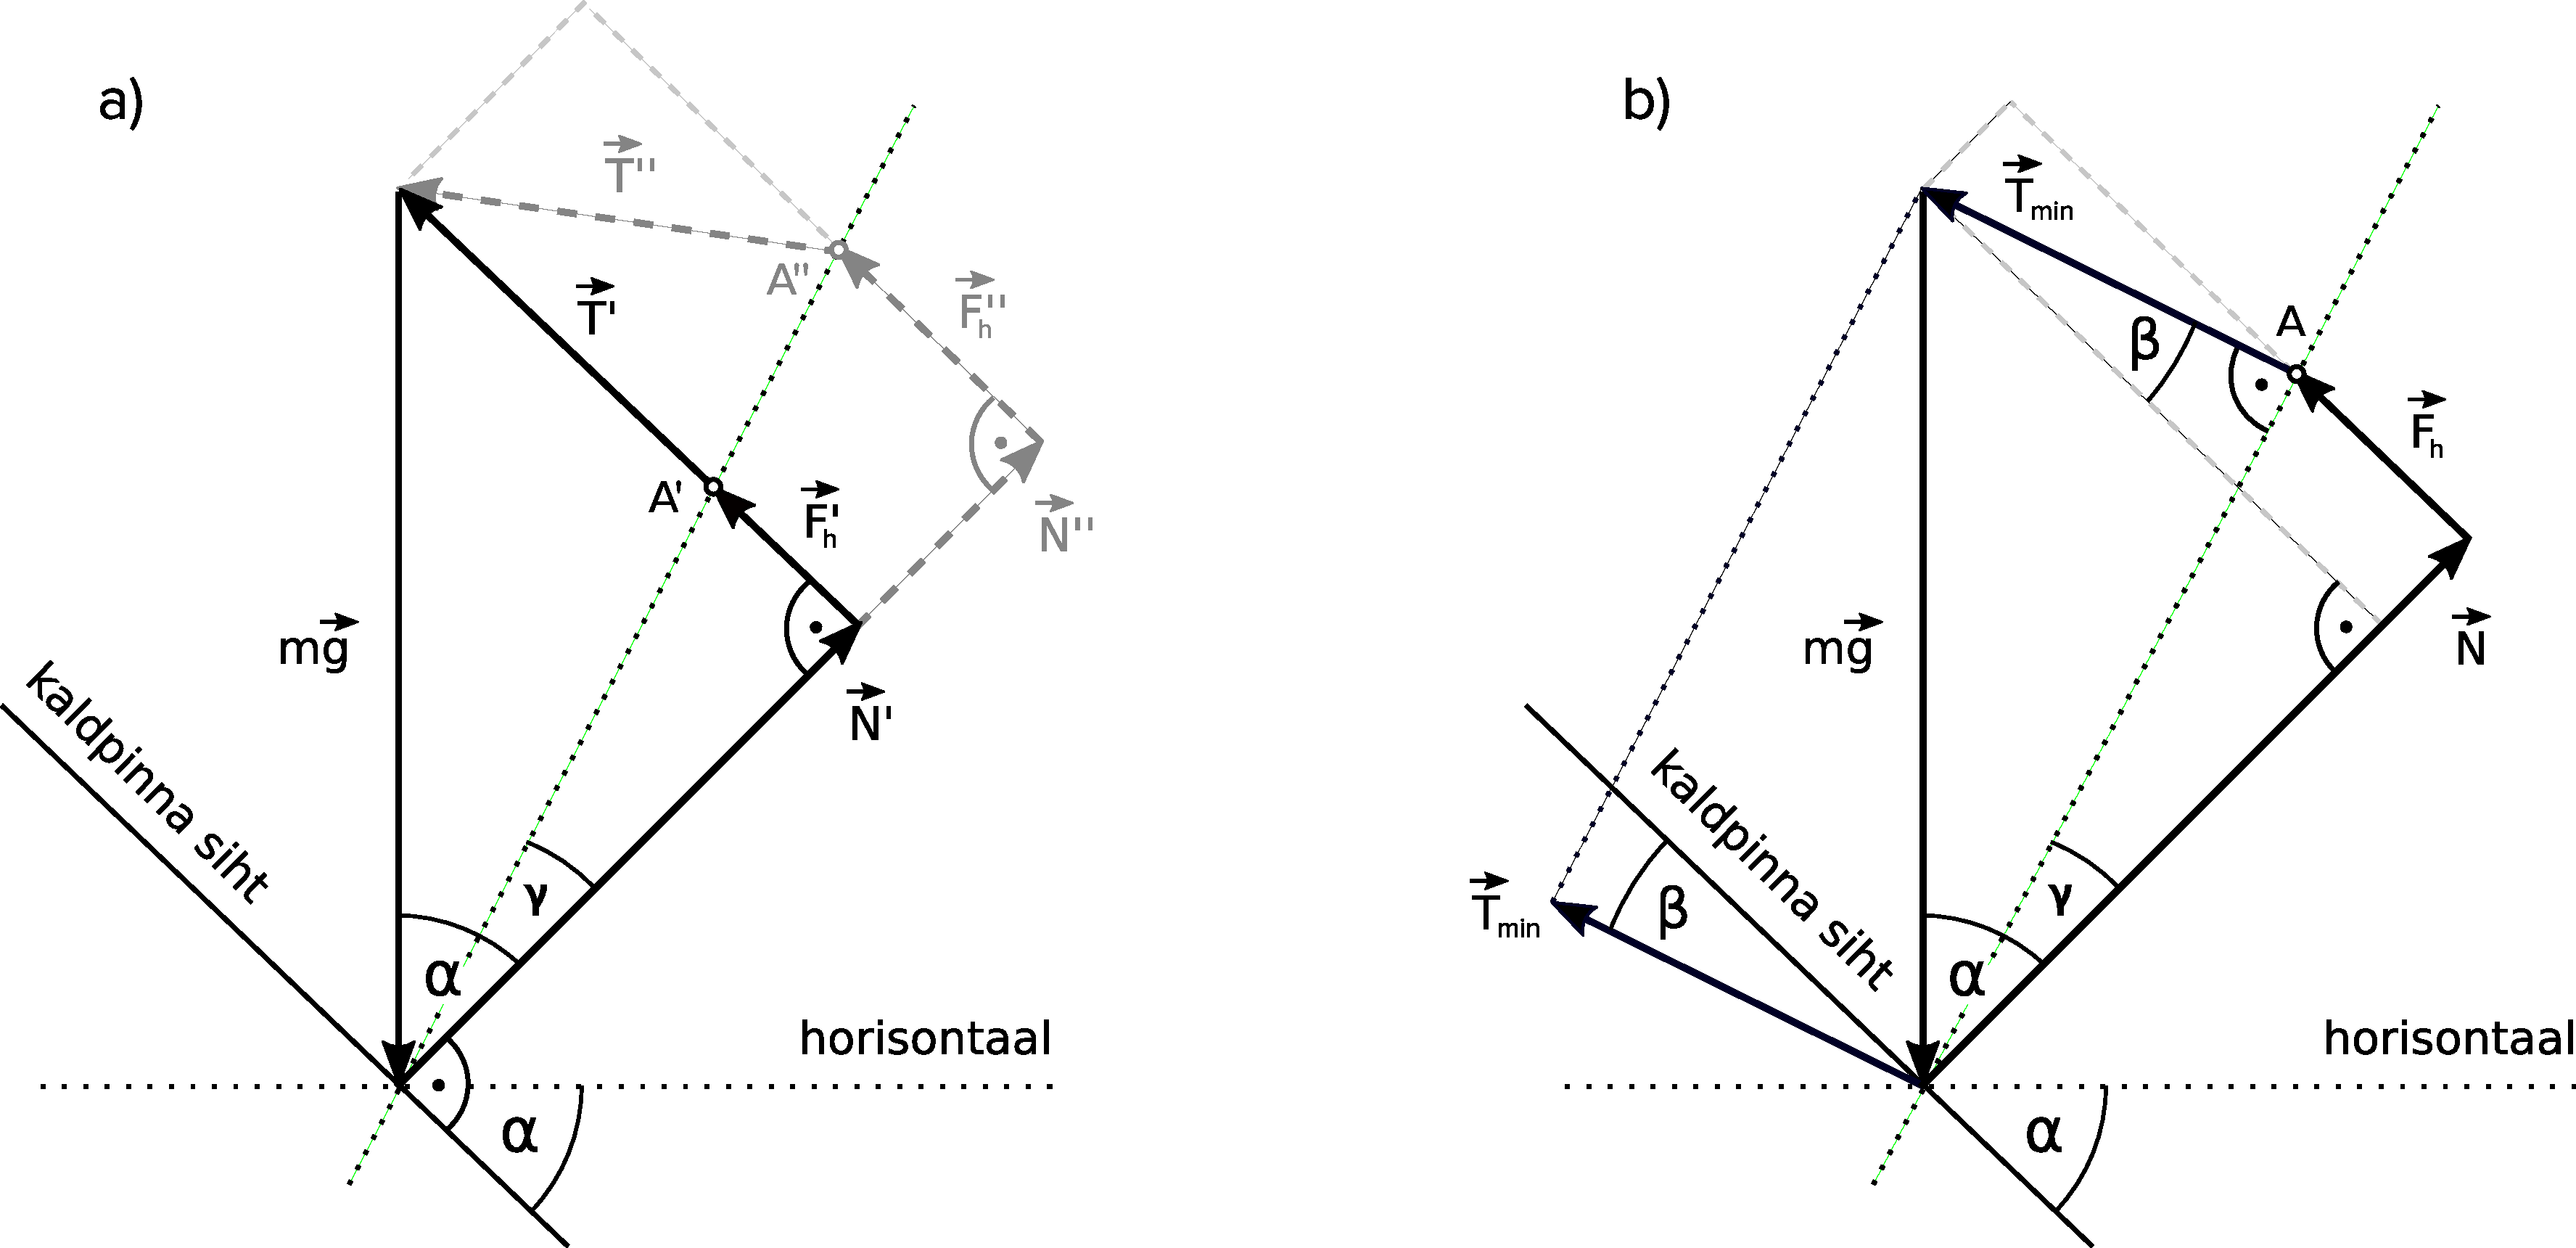
\includegraphics[width=0.9\linewidth]{laev_lahendus_1.pdf}
    %\caption{}
  \end{center}
  \vspace{-0.5cm}
\end{figure}

Vaatleme kõigepealt olukorda, kus köie tõmbejõud mõjub paralleelselt kaldpinnaga. Joonisel a) on sellele olukorrale vastavad jõud tähistatud primmiga. Nüüd on lihtne näha, et võimalikele tasakaaluolekutele vastavad vektordiagrammid saame, kui liigutame punkti A suvaliselt vektoriga $\overrightarrow{N}+\overrightarrow{F}_h$ määratud sihis. Sealjuures paneme tähele, et vektori $\overrightarrow{T}$ pikkus on minimaalne siis, kui see asetseb $\overrightarrow{N}+\overrightarrow{F}_h$ sihiga risti. Selline olukord on kujutatud joonisel b). Sarnaste kolmnurkade võrdlemine annab minimaalsele tõmbele vastava nurga $\beta$ väärtuseks $\beta=\gamma=\arctan\mu$. Samalt vektordiagrammilt saame ka minimaalse tõmbe
\[T_{min}=mg\sin(\alpha-\gamma)=\]
\[=mg\sin(\alpha-\arctan\mu)= mg\frac{\sin\alpha-\mu\cos\alpha}{\sqrt{1+\mu^2}}.\]


\emph{Märkus:} Kui lahendaja eeldab ekslikult, et $\overrightarrow{T}_{min}$ on paralleelne kaldpinnaga ja tuletab sellest lähtuvalt lõppvalemi $T$ jaoks, siis hinnata lahendust
maksimaalselt 4 p. vääriliseks.

\begin{wrapfigure}{r}{0.5\textwidth}
\vspace{-0.5cm}
  \begin{center}
    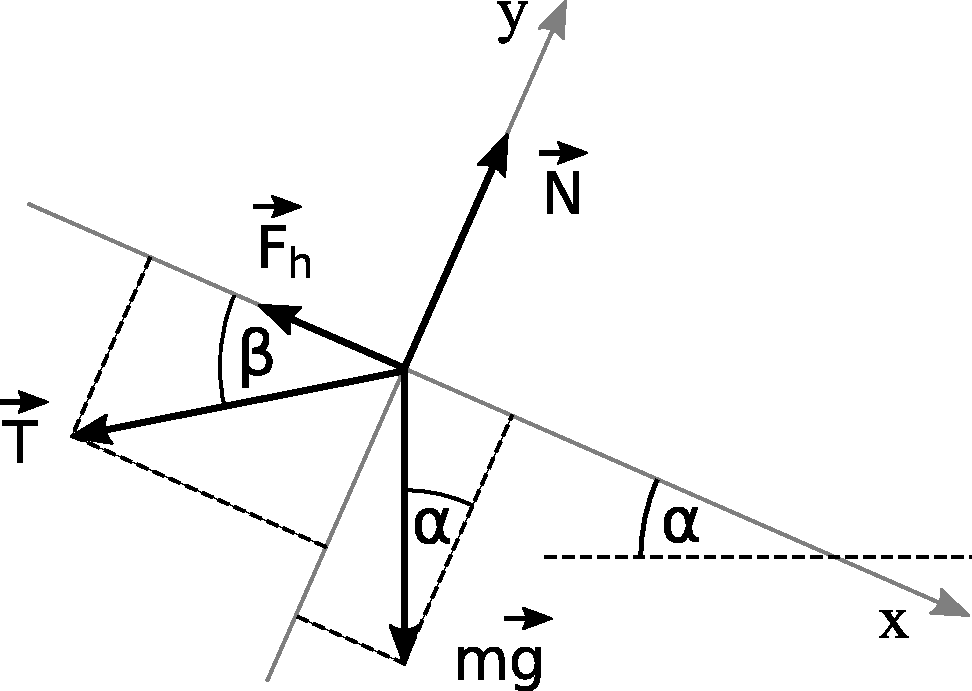
\includegraphics[width=0.8\linewidth]{laev_lahendus_2.pdf}
  \end{center}
  \vspace{-0.5cm}
\end{wrapfigure}
\textbf{Lahendus 2.} \\
Olgu $\beta$ nurk kaldpinna sihi ja tõmbe $T$ sihi vahel. Valime ristkoordinaadistiku selliselt, et $x$-telg asetseb kaldpinna sihis. Kirjutame mõlema koordinaatelje jaoks välja jõudude tasakaalutingimused:
\begin{align*}
  F_x &= mg\sin{\alpha}-T\cos\beta-F_h=0,\\
  F_y &= N-T\sin\beta-mg\cos\alpha=0.
\end{align*}
Teisest võrrandist saame $N=T\sin\beta+mg\cos\alpha$
ja et $F_h =\mu N$, siis asendades need seosed esimesse võrrandisse saame
\[mg\sin\alpha-T\cos\beta-\mu T\sin\beta - \mu mg\cos\alpha=0,\]
millest
\[T=mg\frac{\sin\alpha-\mu\cos\alpha}{\cos\beta+\mu\sin\beta}.\]
Viimane valem annab tasakaalustava tõmbe $T$ suvalise nurga $\beta$ korral, kõik ülejäänud valemis esinevad parameetrid on ülesande tekstis fikseeritud suurused ehk konstandid.
Järelikult võime tõmmet $T$ vaadelda funktsioonina ühest muutujast $\beta$, st $T=T(\beta)$. Edasine ülesanne seisneb selle funktsiooni miinimumi leidmises. On selge, et $T$ on minimaalne siis,
kui nimetajas olev avaldis $\cos\beta+\mu\sin\beta$ on maksimaalne. Maksimumi määramiseks leiame selle avaldise tuletise $\beta$ järgi ja võrdsustame selle nulliga:
\[(\cos\beta+\mu\sin\beta)'=-\sin\beta+\mu\cos\beta=0, \]
millest $\mu=\tan\beta$ ehk $\beta=\arctan\mu$, mis ongi $T$ minimaalsele väärtusele vastav nurk. Asendades selle $T$ avaldisse saame
\[T_{min}=mg\frac{\sin\alpha-\mu\cos\alpha}{\cos(\arctan\mu)+\mu\sin(\arctan\mu)}= mg\frac{\sin\alpha-\mu\cos\alpha}{\sqrt{1+\mu^2}}.\]

\textbf{Hindamisskeem lahendusele 2.} \\
Õiged jõudude tasakaaluvõrrandid õpilase valitud koordinaatsüsteemis koos seletustega või joonisega, kus on näidatud võrranditele vastavad jõud ja nurgad [\textbf{4 p.}]\\
Korrektselt leitud $T$ üldavaldis [\textbf{2 p.}]\\
On aru saadud, et ülesanne taandub funktsiooni $T$ miinimumi leidmisele, ning et selleks tuleb kasutada tuletist. [\textbf{1 p.}]\\
Õigesti leitud tuletis ja sellest saadud miinimumile vastav seos $\mu=\tan\beta$, kus $\beta$ on nurk kaldpinna ja $\overrightarrow{T}_{min}$ vahel [\textbf{3 p.}]\\
Saadud õige lõppavaldis $T_{min}=mg\frac{\sin\alpha-\mu\cos\alpha}{\cos(\arctan\mu)+\mu\sin(\arctan\mu)}$ või sellega ekvivalentne avaldis, mis sisaldab ainult ülesande tekstis antud parameetreid
ja gravitatsioonikiirendust $g$ [\textbf{2 p.}]

\emph{Märkus:} Kui lahendaja eeldab ekslikult, et $\overrightarrow{T}_{min}$ on paralleelne kaldpinnaga ja tuletab sellest lähtuvalt lõppvalemi $T$ jaoks, siis hinnata lahendust
maksimaalselt 4 p. vääriliseks.

\end{document}
